\documentclass{beamer}

\usepackage[utf8]{inputenc}
\usepackage{default}
\usepackage{pslatex}
\usepackage{graphicx}
% \usepackage{algorithmic}
\usepackage{multicol}
\usepackage[french]{babel}

\usetheme{Warsaw}

\title{Comment simuler numériquement la géomorphologie alpine ?}
\subtitle{Sujet de TPE}
\author{Gros Alexis, Manceau Thibaut, Porteries Tristan}
% \logo{
\includegraphics[height=0.5cm]{blender.png}}

\makeindex

\useoutertheme{infolines}

\begin{document}

% Titre
\frame{\titlepage}

% Sommaire
\begin{frame}{Sommaire}
  \begin{multicols}{2}
    \small \tableofcontents
  \end{multicols}
\end{frame}

\section{Les phénomènes géormophologiques}
\subsection{La subduction et l'obduction}
\begin{frame}
  \begin{figure}
    \begin{center}
      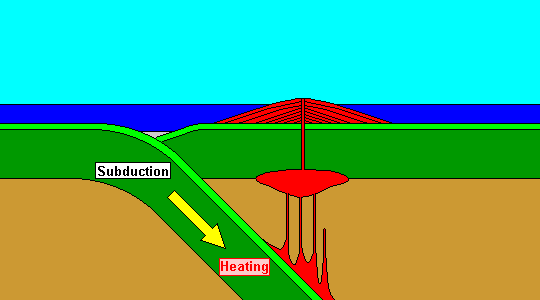
\includegraphics[width=6cm]{Images/subduction.png}
      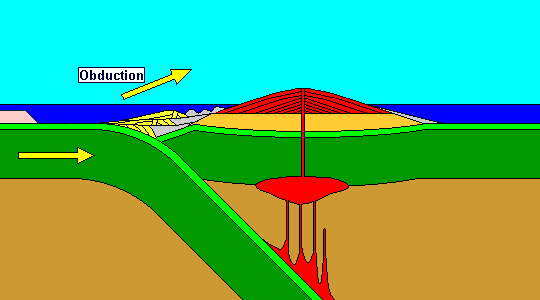
\includegraphics[width=6cm]{Images/obduction.png}
      \caption{A gauche le subduction et à droite l'obduction.}
    \end{center}
  \end{figure}
\end{frame}

\section{Les altérations}
\subsection{Les altérations physiques}
\begin{frame}
  \begin{center}
    \begin{figure}
      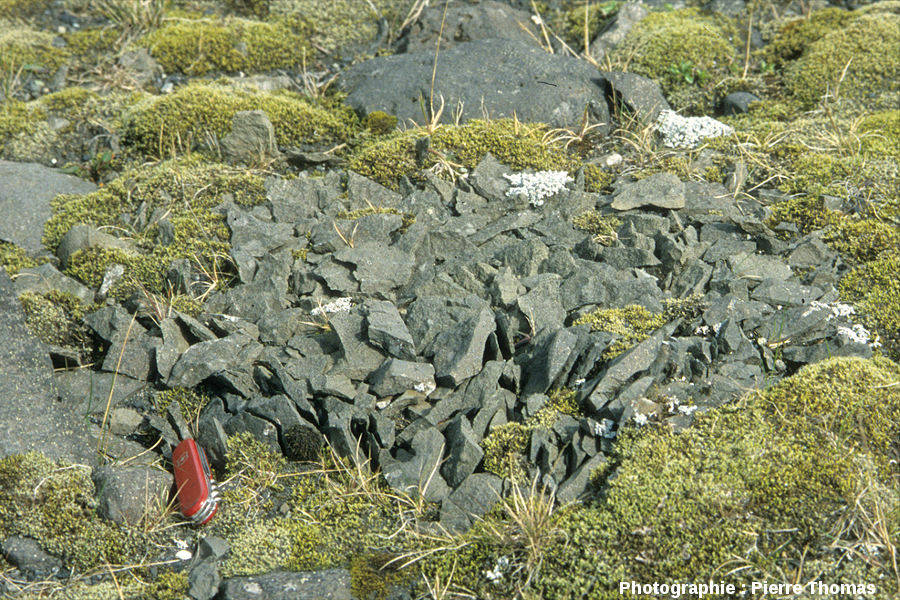
\includegraphics[width=4.5cm]{Images/Diapos/Alteration/Physique/cryoclastie.jpg}
      \caption{Cryoclastie}
    \end{figure}
  \end{center}
  \begin{center}
    \begin{figure}
      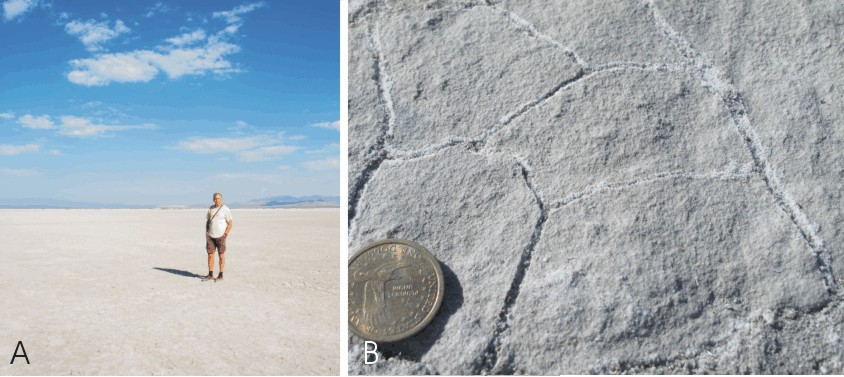
\includegraphics[width=7.4cm]{Images/Diapos/Alteration/Physique/haloclastie3.jpg}
      \caption{Haloclastie}
    \end{figure}
  \end{center}
\end{frame}

\subsection{Les altérations biologiques}
\begin{frame}
  \begin{center}
    \begin{figure}
      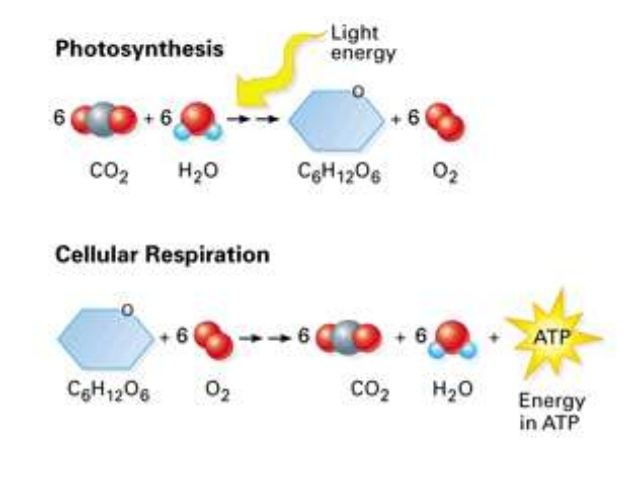
\includegraphics[width=8cm]{Images/Diapos/Alteration/Biologique/biology-unit-3-cell-energy-cellular-respiration-notes-3-638.jpg}
      \caption{Schéma de la respiration cellulaire.}
    \end{figure}
  \end{center}
\end{frame}

\subsection{Les altérations chimiques}
\begin{frame}
  \begin{center}
    \begin{figure}
      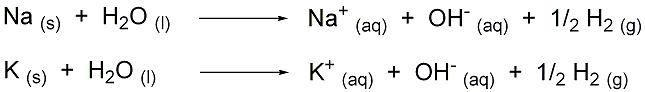
\includegraphics[width=7cm]{Images/Diapos/Alteration/Chimiques/hydrolyse.png}
      \caption{Hydratation de molécules de sodium et de potassium.}
    \end{figure}
  \end{center}
  \begin{center}
    \begin{figure}
      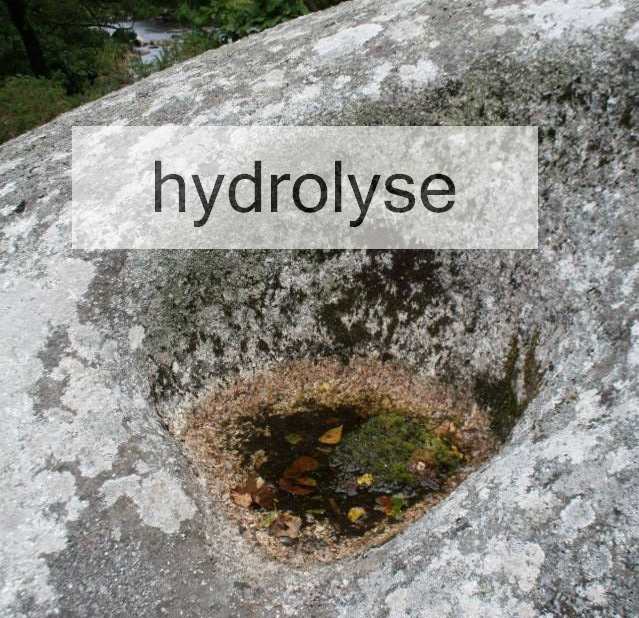
\includegraphics[width=5cm]{Images/Diapos/Alteration/Chimiques/hydrolyse.jpeg}
    \end{figure}
  \end{center}
\end{frame}

\section{L'érosion}
\subsection{L'érosion éolienne}
\begin{frame}
  \begin{figure}[h]
    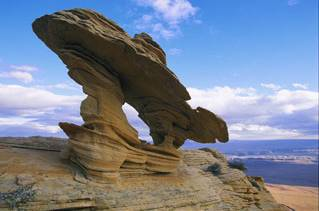
\includegraphics[width=5cm]{Images/Diapos/Erosion/Eolienne/Vent.jpg}
    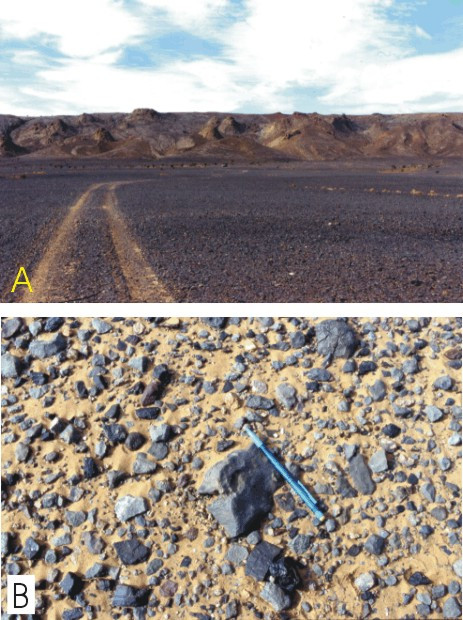
\includegraphics[width=5cm]{Images/Diapos/Erosion/Eolienne/Vent2.jpg}
  \end{figure}
\end{frame}

\subsection{Le ruissellement et l'érosion fluviale}
\begin{frame}
  \begin{figure}
    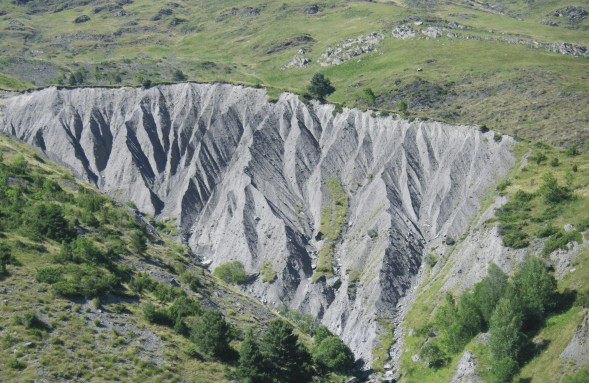
\includegraphics[width=5cm]{Images/Diapos/Erosion/Fluviale/bad_lands.jpg}
    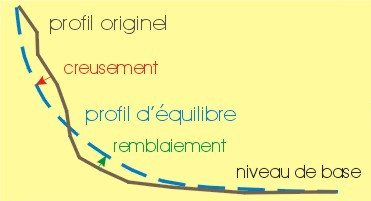
\includegraphics[width=6cm]{Images/Diapos/Erosion/Fluviale/n_base.jpg}
    \caption{Ruissellement et érosion verticale}
  \end{figure}
  \begin{center}
    \begin{figure}
      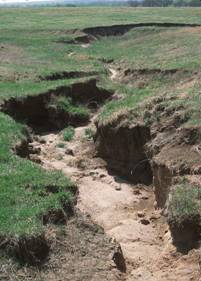
\includegraphics[width=2cm]{Images/Diapos/Erosion/Fluviale/solixfluxion.jpg}
      \caption{Solifluxion}
    \end{figure}
  \end{center}
\end{frame}

\subsection{L'érosion karstique}
\begin{frame}
  \begin{center}
    \begin{figure}[h]
      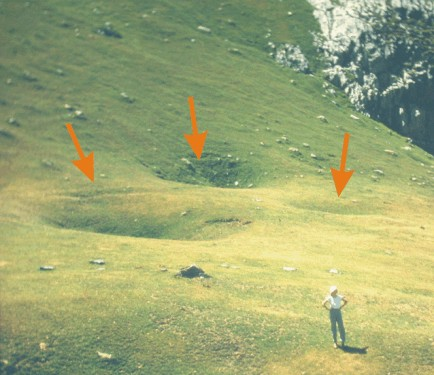
\includegraphics[width=5.35cm]{Images/Diapos/Erosion/Karstique/dolines.jpg}
      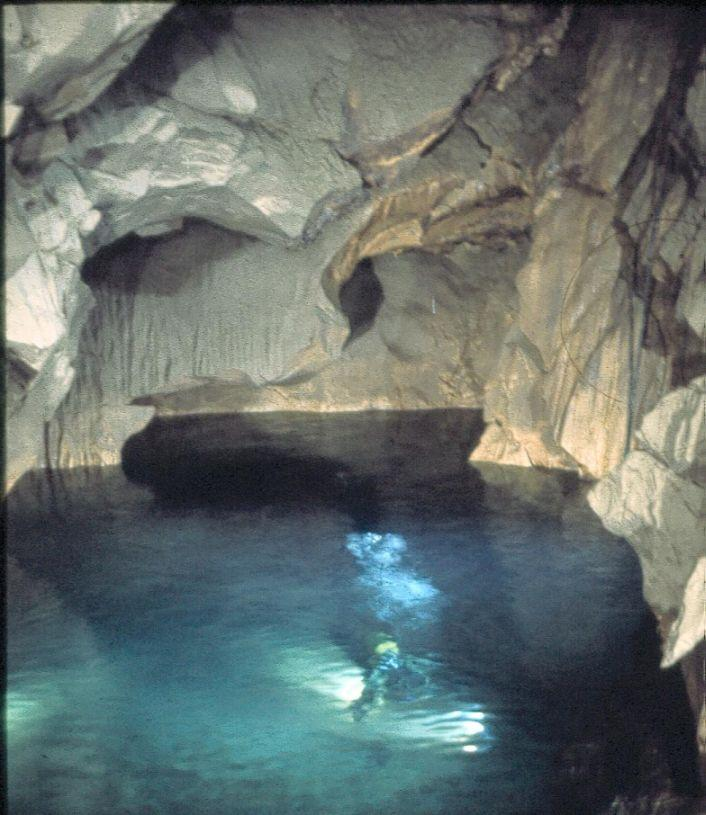
\includegraphics[width=4cm]{Images/Diapos/Erosion/Karstique/erosion-karstique-fig04.jpg}
      \caption{Dolines et grotte souterraine dus à l'érosion karstique.}
    \end{figure}
  \end{center}
\end{frame}

\subsection{L'érosion glaciaire}
\begin{frame}
  \begin{center}
    \begin{figure}
      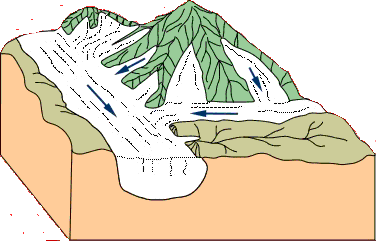
\includegraphics[width=8cm]{Images/Diapos/Erosion/Glaciaire/Erosion_glaciaire_Bourque4B.png}
      \caption{Schéma de l'érosion glaciaire}
    \end{figure}
  \end{center}
\end{frame}

\subsection{L'érosion marine}
\begin{frame}
  \begin{center}
    \begin{figure}
      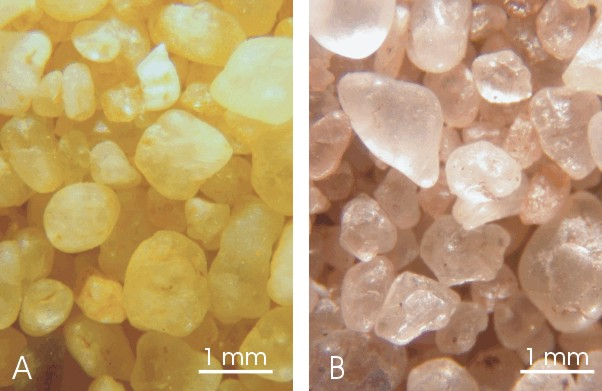
\includegraphics[width=5cm]{Images/Diapos/Erosion/marine/A_vent_B_mer.jpg}
      \caption{Grains de sable exposés (A) au vent (B) aux embruns.}
      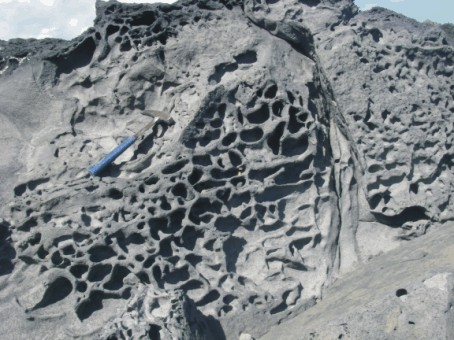
\includegraphics[width=4cm]{Images/Diapos/Erosion/marine/taffoni.jpg}
      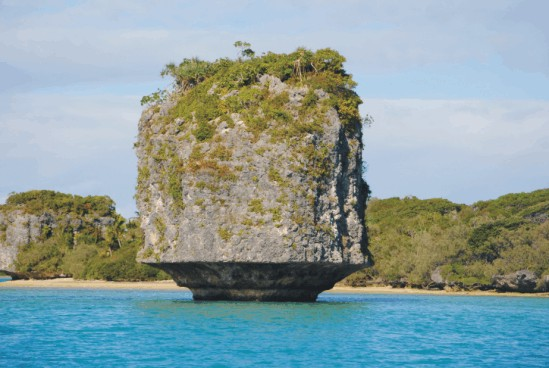
\includegraphics[width=4.5cm]{Images/Diapos/Erosion/marine/upi.jpg}
      \caption{A gauche Taffoni et à droite encoche d'érosion marine.}
    \end{figure}
  \end{center}
\end{frame}

\section{Le système cellulaire}
\begin{frame}
  \begin{figure}
    \begin{center}
      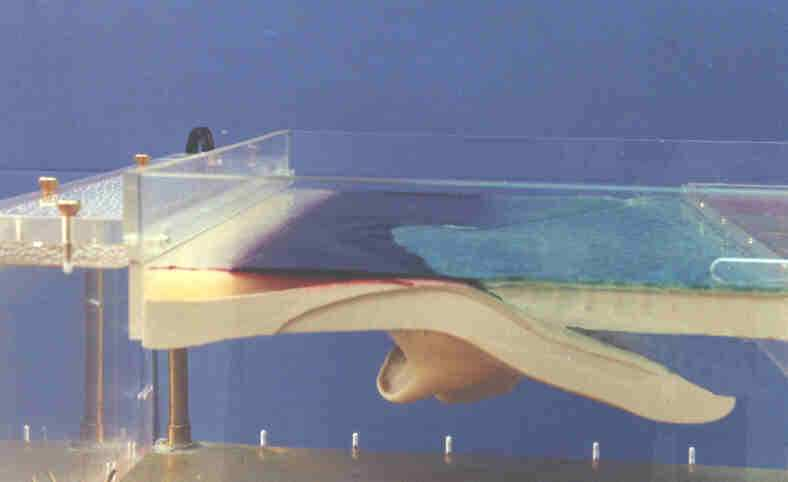
\includegraphics[width=8cm]{simulation_physique.png}
      \caption{Simulation physique d'une subduction à l'aide de matières molles.}
    \end{center}
  \end{figure}
\end{frame}

\subsection{Approche simplifiée pour le jeu vidéo}
\begin{frame}
    Approximation avec des algorithmes mathématique sans nécessités physiques~:
  \begin{itemize}
      \item La fonction du bruit de Perlin~;
      \item Biomes avec les polygones de Voronoi~;
      \item interpolation avec la courbe de Bézier~;
      \item Calcul des chemins d'érosion par l’enchaînement~;
      \item Possibilité d'édition par l'utilisateur.
  \end{itemize}
\end{frame}

\subsection{Le système cellulaire}
\begin{frame}
  \begin{center}
    \begin{figure}
      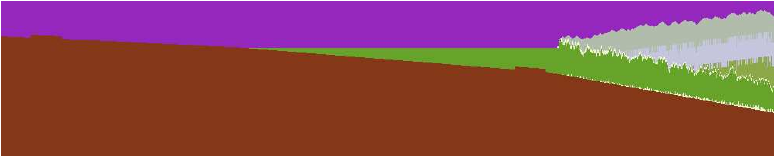
\includegraphics[width=10cm]{Images/3100_cell.png}
      \caption{Simulation par automate cellulaire après 3100 itérations.}
    \end{figure}
    \begin{figure}
      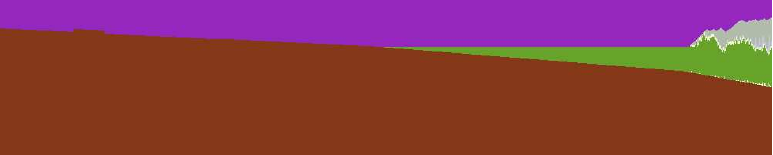
\includegraphics[width=10cm]{Images/7100_cell.png}
      \caption{Simulation par automate cellulaire après 7100 itérations.}
    \end{figure}
  \end{center}
\end{frame}

\subsection{Simulation par voxels}
\begin{frame}
  \begin{center}
    \begin{itemize}
      \item Simulation par voxels
      \item Approche cellulaire de la simulation
    \end{itemize}
    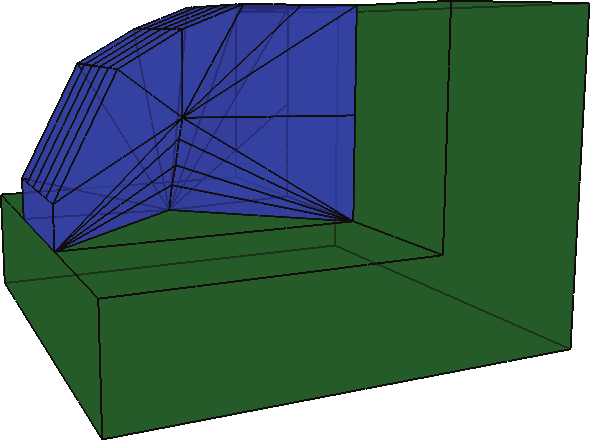
\includegraphics[width=8cm]{kk.png}
  \end{center}
\end{frame}

\subsection{Les cellules}
\begin{frame}
  Cellule : le plus petit élément incompressible de la simulation, représenté par une sphère de diamètre 1. \smallbreak
  Propriétés mutables :
  \begin{itemize}
   \item vélocité~;
   \item position~;
   \item cellules adjacentes.
  \end{itemize}
  Propriétés immuables :
  \begin{itemize}
   \item plaque tectonique.
  \end{itemize}
  Disposition en nid-d'abeille au lancement de la simulation.
  \begin{center}
    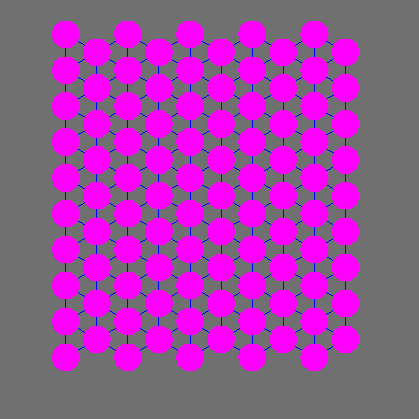
\includegraphics[width=4cm]{Images/hexagone.png}
  \end{center}
\end{frame}

\subsection{La propagation par fronts}
\begin{frame}
  Propagation par front, l’ancien front crée le nouveau. Le premier front ne contient que la cellule en collision.
  Chaque cellule du front interagit avec les cellules qui précèdent le front.
  \begin{figure}
    \begin{center}
      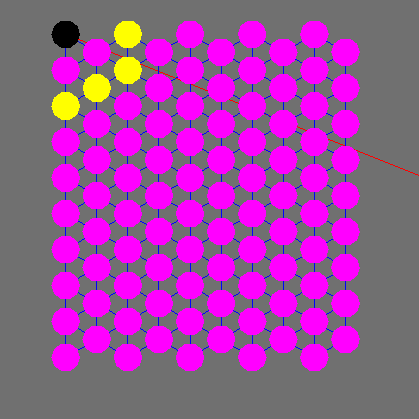
\includegraphics[width=2.5cm]{Images/front_1.png}
      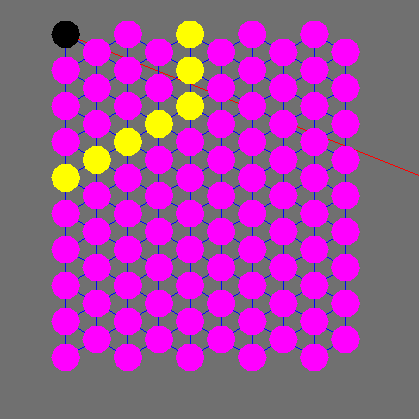
\includegraphics[width=2.5cm]{Images/front_2.png}
      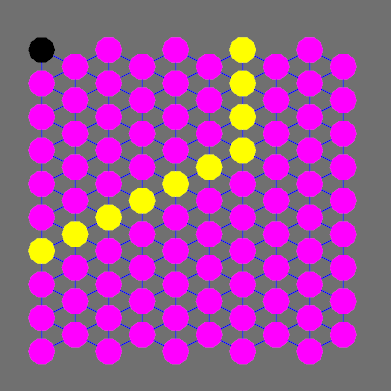
\includegraphics[width=2.5cm]{Images/front_3.png}
    \end{center}
    \begin{center}
      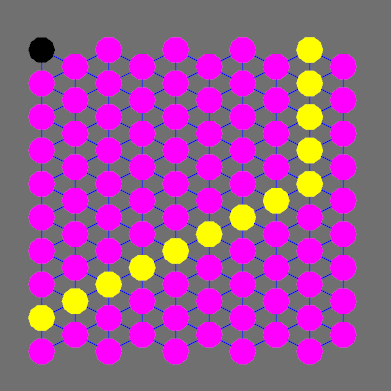
\includegraphics[width=2.5cm]{Images/front_4.png}
      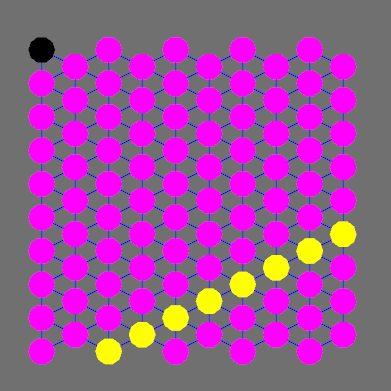
\includegraphics[width=2.5cm]{Images/front_5.png}
      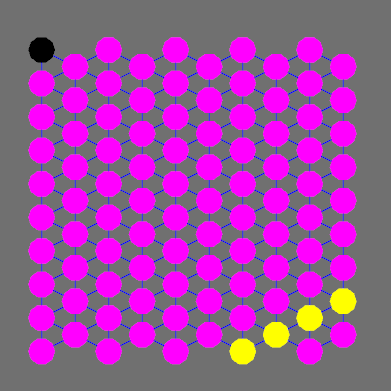
\includegraphics[width=2.5cm]{Images/front_6.png}
    \end{center}

    \caption{Bleu : liens entre cellules, Violet : cellules inactives, Noir : cellule de collision, Jaune : cellules appartenant au front.}
  \end{figure}
\end{frame}

\begin{frame}
  Utilisation d'un calque pour chaque cellule en collision. Fusion des calques avant le déplacement des cellules.
  \begin{figure}
    \begin{center}
      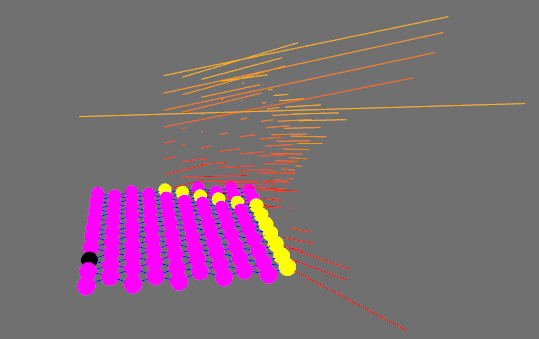
\includegraphics[width=6cm]{Images/layer.png}
    \end{center}
    \caption{Du rouge vers le jaune les différentes vélocités par cellules et par collisions.}
  \end{figure}
\end{frame}


\section{Les interactions entre cellules}
\subsection{Loi du centre instantané de rotation}
\begin{frame}
  \begin{multicols}{2}
    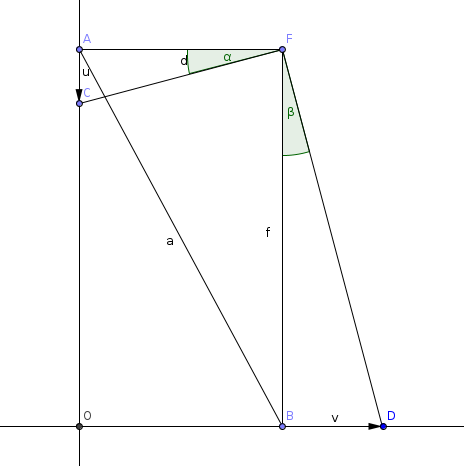
\includegraphics[width=5cm]{Images/geogebra_1.png}
    \vfill
    \columnbreak
    $\overrightarrow{u} = $ vélocité verticale \smallbreak
    $\overrightarrow{v} = $ vélocité horizontale \smallbreak
    $\alpha = \beta = $ rotation autour de F \smallbreak
    $||\overrightarrow{u}|| = \alpha \times d$ \smallbreak
    $||\overrightarrow{v}|| = \alpha \times f$ \smallbreak
    $\alpha = \frac{||\overrightarrow{u}||}{d}$ \smallbreak
  \end{multicols}
\end{frame}

\begin{frame}
  \begin{multicols}{2}
    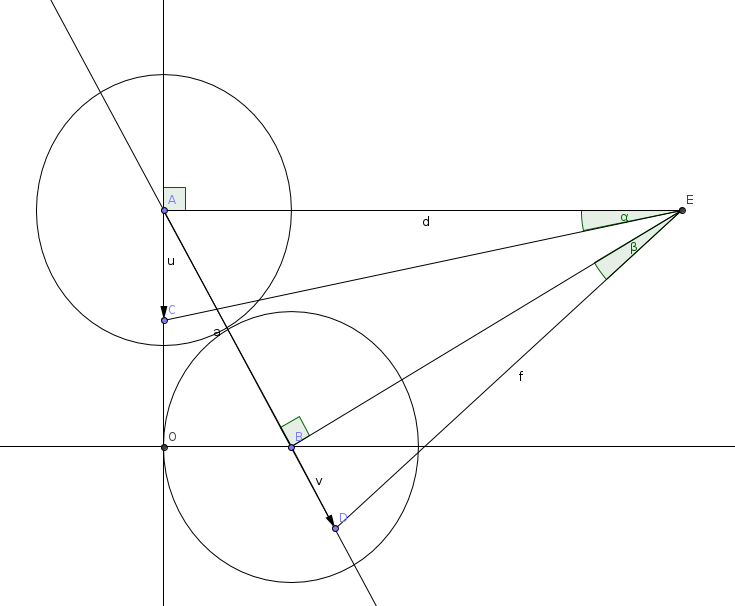
\includegraphics[width=6cm]{Images/geogebra_2.png}
    \vfill
    \columnbreak
    Si $(\overrightarrow{v}, \overrightarrow{u}) = 0$ \smallbreak
    $\overrightarrow{v} = \overrightarrow{u}$ \smallbreak
    $d = f = \infty$ \smallbreak
    Si $(\overrightarrow{u}, \overrightarrow{v}) = \frac{\pi}{2}$ \smallbreak
    $f = 0$ \smallbreak
    $\overrightarrow{v} = \overrightarrow{0}$
  \end{multicols}
\end{frame}

\begin{frame}
  \begin{figure}
    \begin{center}
      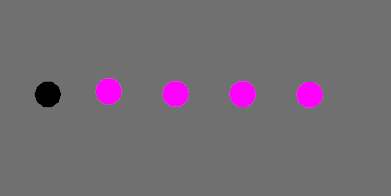
\includegraphics[width=3.5cm]{Images/cir_1.png}
      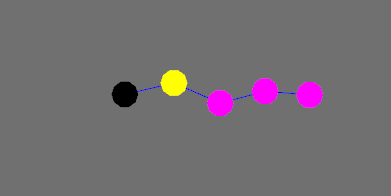
\includegraphics[width=3.5cm]{Images/cir_2.png}
      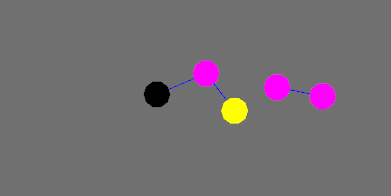
\includegraphics[width=3.5cm]{Images/cir_3.png}
    \end{center}
    \begin{center}
      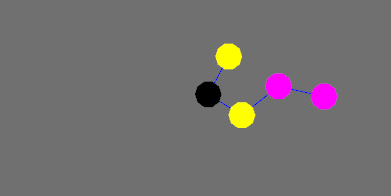
\includegraphics[width=3.5cm]{Images/cir_4.png}
      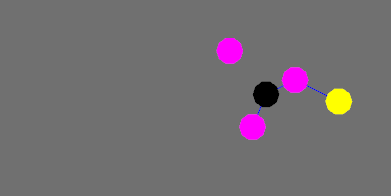
\includegraphics[width=3.5cm]{Images/cir_5.png}
      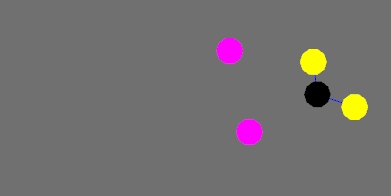
\includegraphics[width=3.5cm]{Images/cir_6.png}
    \end{center}
    \caption{6 échantillons de compressions avec le CIR.}
  \end{figure}
\end{frame}



\subsection{La loi de Hooke et le module de Young}
\begin{frame}
  \begin{center}
    $\sigma = E \times \varepsilon$
  \end{center}
  $\sigma = $ La contrainte appliquée sur le matériau (en Pa). $E = $ Le module de Young pour le matériau étudié (en Pa). $\varepsilon = $ Coefficient de déformation (en $\%$). \smallbreak
  Module de Young :
  \begin{itemize}
    \item Granite : 60 GPa ;
    \item Calcaire : 20 à 70 GPa.
  \end{itemize}
  \smallbreak
  \begin{center}
    $\varepsilon = \frac{x_{max}}{\sqrt{x}}$
  \end{center}
  $x_{max} = $ La distance à respecter entre deux cellules. $x = $ La distance entre les deux cellules. \smallbreak
  \begin{center}
    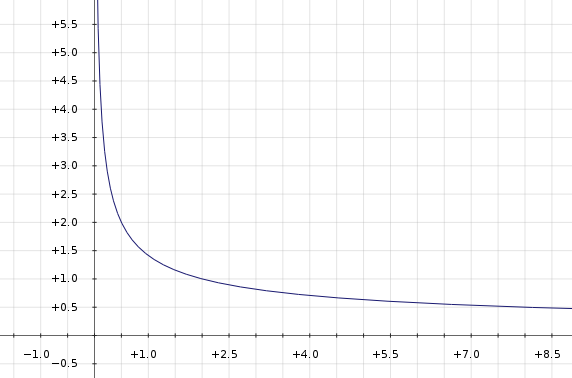
\includegraphics[width=3cm]{Images/compression_kmplot.png}
  \end{center}
\end{frame}

\begin{frame}
  \begin{figure}
    \begin{center}
      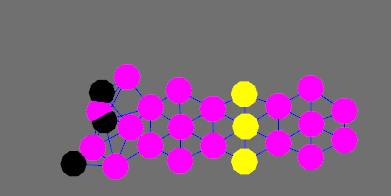
\includegraphics[width=6cm]{Images/no_compression.png}
      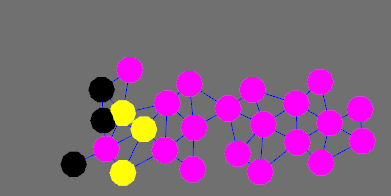
\includegraphics[width=6cm]{Images/compression.png}
    \end{center}
    \caption{A gauche simulation sans compression et à droite avec compression.}
  \end{figure}
\end{frame}


\subsection{La loi de Coulomb}
\begin{frame}
  \begin{figure}
    \begin{center}
      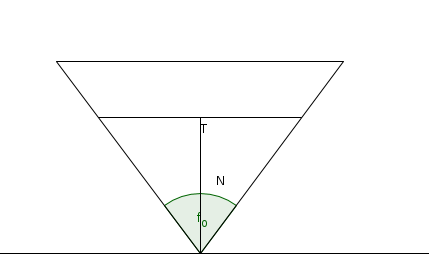
\includegraphics[width=5cm]{Images/friction.png}
    \end{center}
    \caption{Le cône représentant la force maximale possible avant un glissement.}
  \end{figure}
  \begin{center}
    $T_0 = f_0 \times N$
  \end{center}
  Si $T > T_0$ : glissement. Sinon friction. \smallbreak
  Où $T = $ force tangentielle appliquée à la cellule, $N = $ la pression entre les cellules et $f_0 = $ le coefficient d'adhérence.
\end{frame}

\section{Les Améliorations possibles}
\begin{frame}
  Améliorations :
  \begin{itemize}
    \item implémenter l'érosion ;
    \item utilisation de la loi de Hooke et du module de Young~;
    \item utilisation d'un modèle avec friction grâce a la loi de Coulomb~;
    \item implémentation de l'inertie des cellules en fonction de leur masse.
  \end{itemize}
\end{frame}

\section{Conclusion}
\begin{frame}
 
\end{frame}


\end{document}
